\section{Detailed Experiments}\label{sec:detailed-exprs}

\subsection{Variational Autoencoder Layer}\label{subsec:vae-layer-detailed-exprs}

We set the VAE layer with parameters $2048$, $256$, and $2048\times 4$, and trained it on a specifically tidied Open Thought dataset.
The learning rate is set to \num{1e-3}, using the Adam optimizer~\citep{Kingma2014-fu} with batch size $20$.
The training process and loss in $15$ epochs are shown in Figure~\ref{fig:vae-training}.

\begin{figure}[htbp]
    \centering
    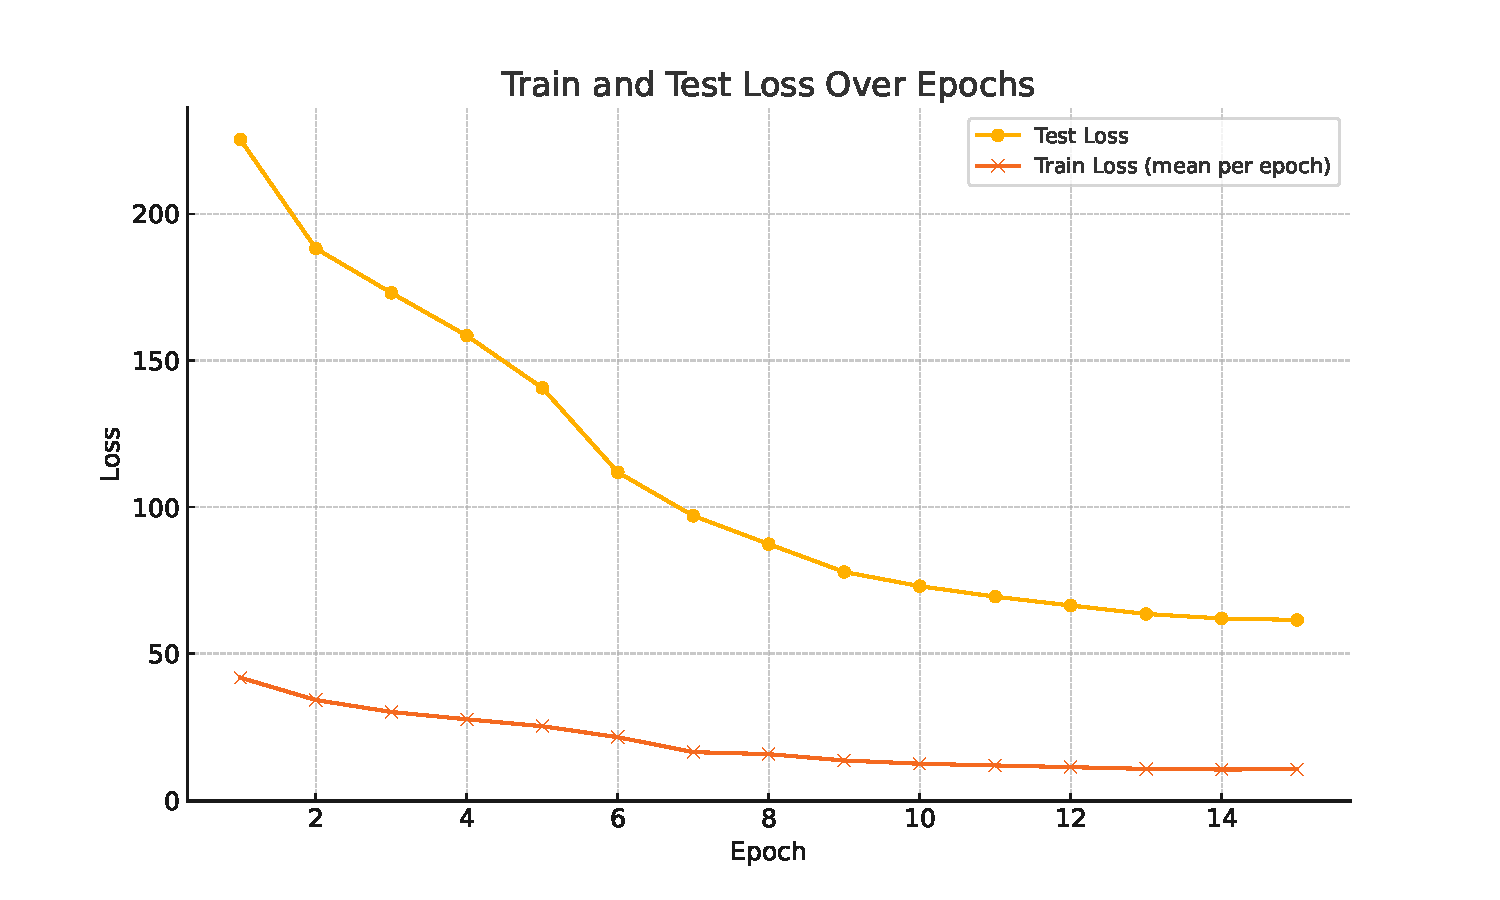
\includegraphics[width=0.6\textwidth]{./figures/vae_train_test_loss_plot}
    \caption{The training process of the VAE layer.
    The reconstruction error of the hidden state vector calculates the loss.
    The training process is stable and converges quickly.}
    \label{fig:vae-training}
\end{figure}